\documentclass[12pt, a4paper]{article}
\usepackage[utf8]{inputenc}
\usepackage[russian]{babel}
\usepackage[pdftex]{graphicx, color}
\usepackage{amsmath}
\usepackage{amsfonts}
\usepackage{amssymb}
\usepackage{amsthm}
\usepackage[left=2cm,right=1.5cm,top=1.5cm,bottom=2cm]{geometry}
\usepackage{indentfirst}
\usepackage{hyperref}

\usepackage{pbox}

\usepackage{setspace}
\onehalfspacing
\graphicspath{{pic/}}

\begin{document}

	\thispagestyle{empty}

	\begin{singlespace}
	\begin{titlepage}
		\begin{center}
			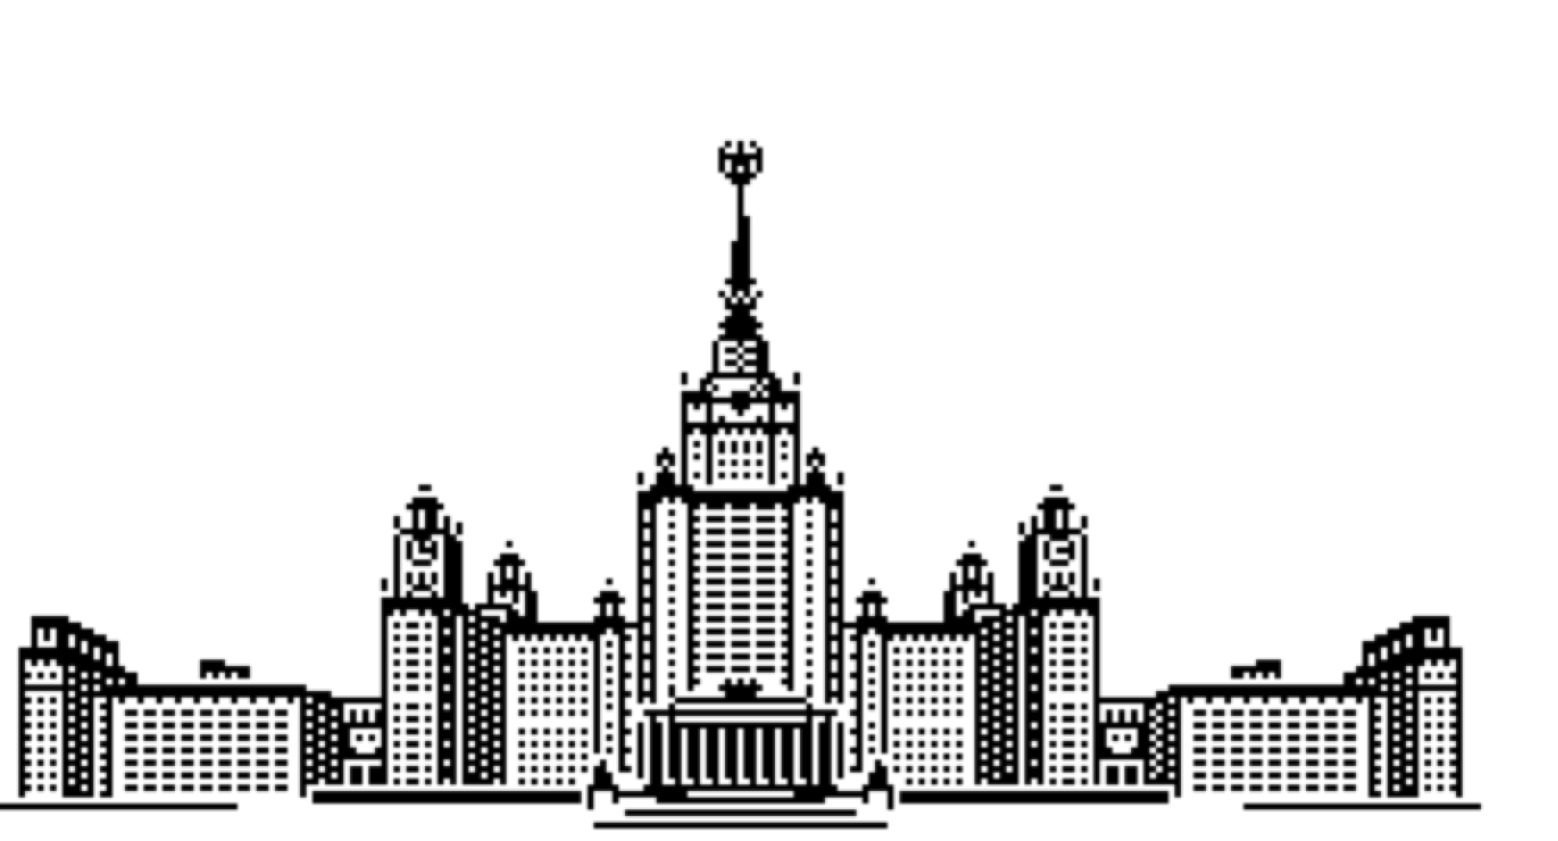
\includegraphics[height = 3cm]{msu.png}

			{\scshape Московский государственный университет имени М.~В.~Ломоносова}\\
			Факультет вычислительной математики и кибернетики\\
			\centerline{\hfill\hrulefill\hrulefill\hrulefill\hrulefill\hfill}

			\vfill

			{\LARGE Отчет к Лабораторной работе \textnumero1: \\ Подсчет монеток на изображении}

			\vspace{1cm}

		\end{center}

		\vfill
		\begin{flushright}
			\textit{Студент 3 курса ВМК (317 группа):}\\
				Оспанов А.М.

			\vspace{5mm}

		\end{flushright}

		\vfill

		\begin{center}
		Москва, 2015
		\end{center}
	\end{titlepage}
	\end{singlespace}

	\tableofcontents

	\newpage
	\section{Введение}
		Данный отчет был написан по дисциплине ``Обработка и распознавание изображений'' студентом 317 группы Оспановым Аятом.

		В данной работе нужно было реализовать алгоритм для подсчета монеток на изображении. Для этого использовались морфологические методы обработки изображений. В качесте языка программирования использовался Python версии 2 с библиотекой OpenCV.

	\newpage
	\section{Основная часть}
		\subsection{Исследование изображений}

			Перед тем, как начать писать код, надо узнать информацию о картинках. В ходе исследований стало известно, что картинки не подчиняются под один закон, т.е. не одинаково распределено освещение, картинки имеют разные фоны и т.д. Но так же был замечен интресный факт при рассмотрении трех каналов картинок: если фон имеет темный цвет, то для бинаризации хорошо подходит красный канал, если фон светлый - то синий. Это можно увидеть из следующих картинок:

			\begin{center}
				Для темного фона

				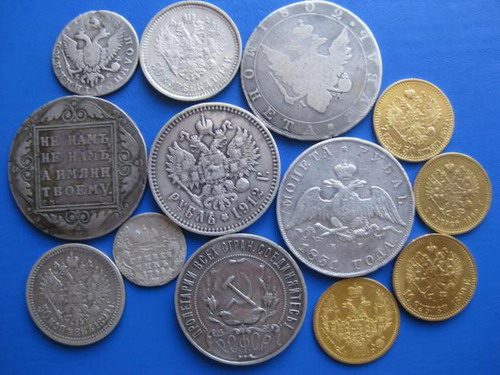
\includegraphics[height=5cm]{Money_1.png}

				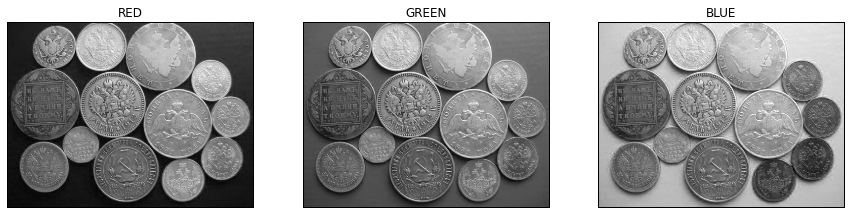
\includegraphics[width=15cm]{1.png}

				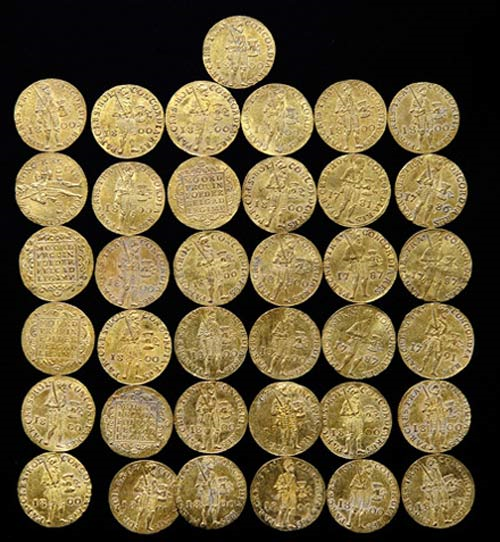
\includegraphics[height=5cm]{Money_8.png}

				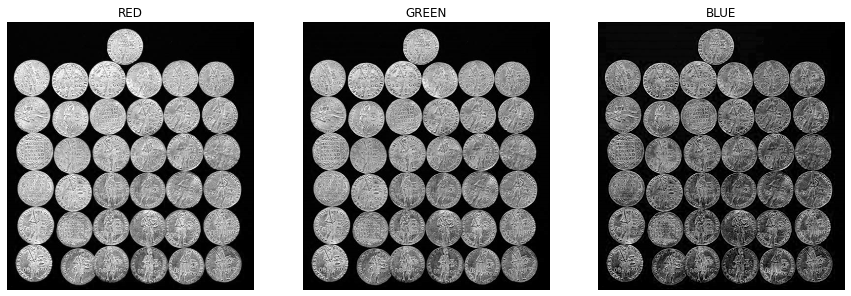
\includegraphics[width=15cm]{8.png}
			\end{center}

			\newpage
			\begin{center}
				Для светлого фона

				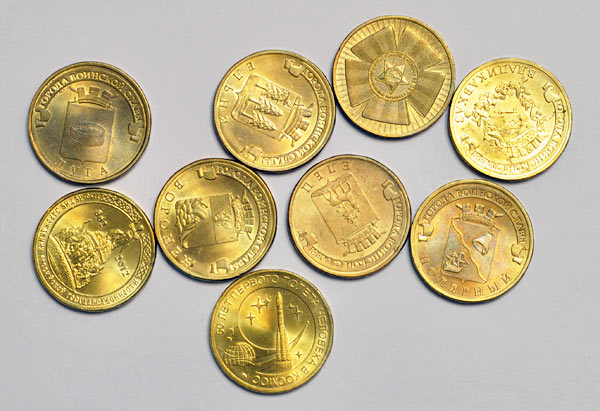
\includegraphics[height=5cm]{Money_2.png}

				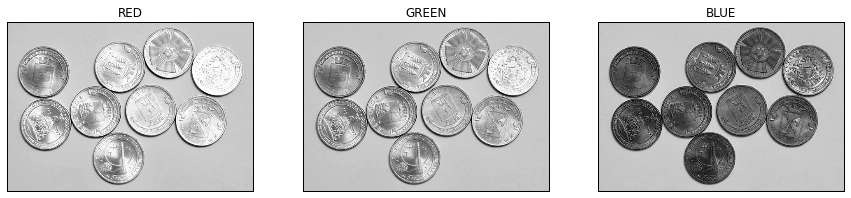
\includegraphics[width=15cm]{2.png}

				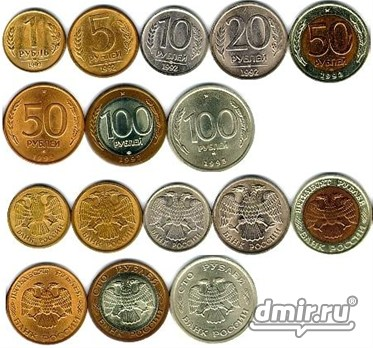
\includegraphics[height=5cm]{Money_3.png}

				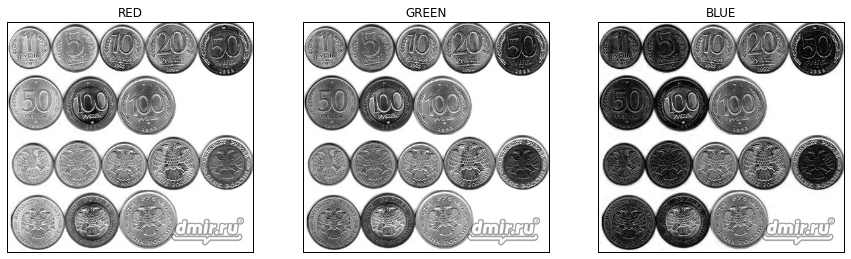
\includegraphics[width=15cm]{3.png}
			\end{center}

		\newpage
		\subsection{Обработка изображений}
			После того, как выяснили характеристики изображений, начнем обработку. Всегда все начинается с бинаризации:
			\begin{center}
				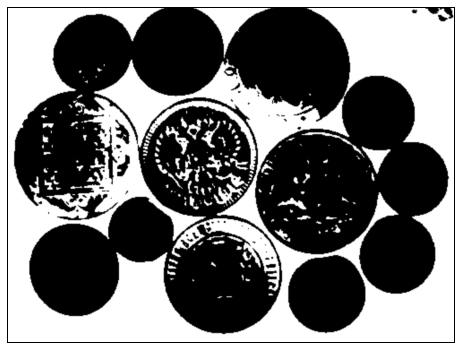
\includegraphics[width=8cm]{Money_1_bin.png}
			\end{center}
			
			Бинаризация делалась адаптивным методом из библиотеки OpenCV: \\
			функция adaptiveThreshold

			Затем комбинации открытий и закрытий (или, что то же самое, дилатация и эрозия):
			
			\begin{center}
				Открытие с эллипсоидальным ядром первого радиуса:

					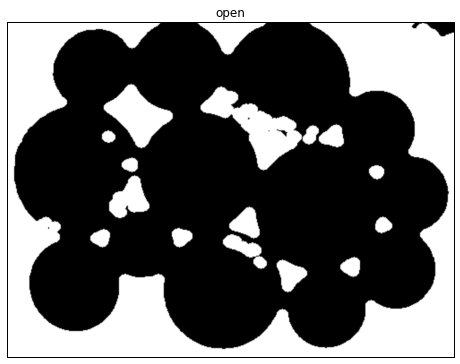
\includegraphics[width=8cm]{open.png}

				Закрытие с эллипсоидальным ядром первого радиуса:

					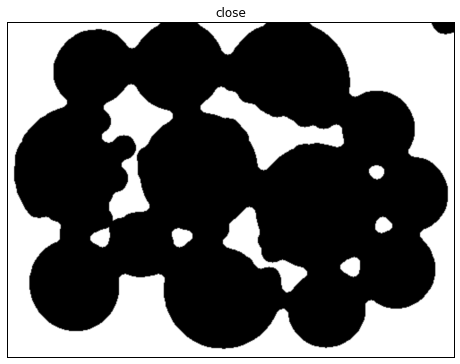
\includegraphics[width=8cm]{close.png}

				\newpage
				Закрытие с эллипсоидальным ядром второго радиуса:

					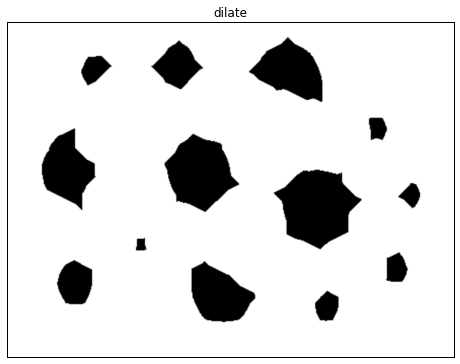
\includegraphics[width=8cm]{dilate.png}

				Открытие с эллипсоидальным ядром второго радиуса:

					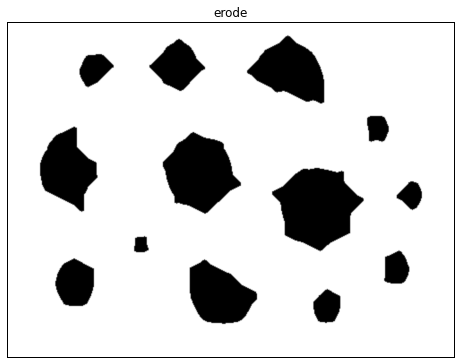
\includegraphics[width=8cm]{erode.png}

				Закрытие с квадратным ядром:

					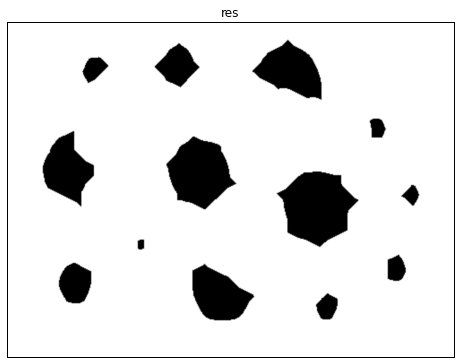
\includegraphics[width=8cm]{dilate_rect.png}		
			\end{center}

			Открытие и закрытие делались следующими функциями: morphologyEx, erode, dilate.

			Радиусы выбирались с целью покрыть этим алгоритмом большее число картинок. Т.к. картинки имеют разные характеристики, то не удается получить единый алгоритм для всех картинок сразу. В ходе исследований выяснилось, что оптимальные параметры следующие:
			\begin{center}
			\begin{tabular}{c c c}
				{\bf Преобразование} & {\bf Ядро} & {\bf Радиус (повторения)} \\
				Первое открытие & Эллипс & 13 (1)\\
				Первое закрытие & Эллипс & 25 (1)\\
				Второе закрытие & Эллипс & 7 (10) \\
				Второе открытие & Эллипс & 5 (1) \\
				Третье закрытие & Квадрат & 7 (1) \\
			\end{tabular}
			\end{center}

			После того, как монеты отделились на компоненты связности, считаем эти компоненты связности. При этом не считаются компоненты, прилегающие к краям. Для этого использовалась функция findContours которая находит контуры и далее остается просто подсчитать количество этих контуров.

	\newpage
	\section{Заключение}

		Данный алгоритм сработал на всех изображениях, кроме 5, 13, 14 изображений, при хорошем подборе констант. Результаты можно увидеть в следующей таблице:

		\begin{center}
		\begin{tabular}{c c}
			{\bf Бинарное изображение} & {\bf Конечное изображение} \\
			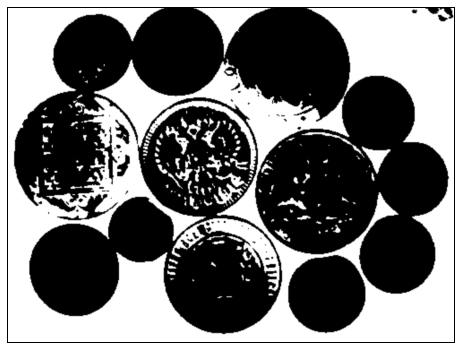
\includegraphics[width=8cm]{Money_1_bin.png} & 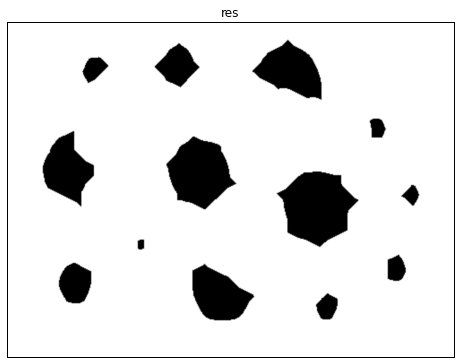
\includegraphics[width=8cm]{Money_1_res.png} \\
			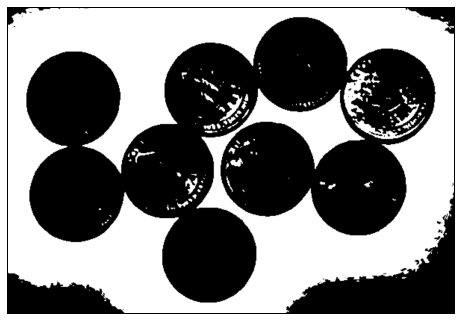
\includegraphics[width=8cm]{Money_2_bin.png} & 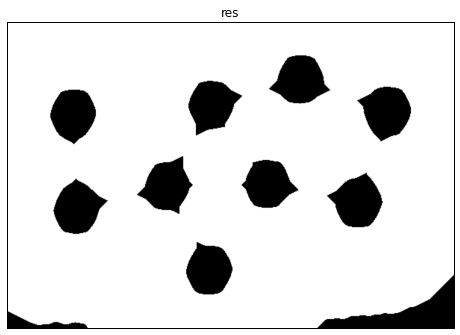
\includegraphics[width=8cm]{Money_2_res.png} \\
			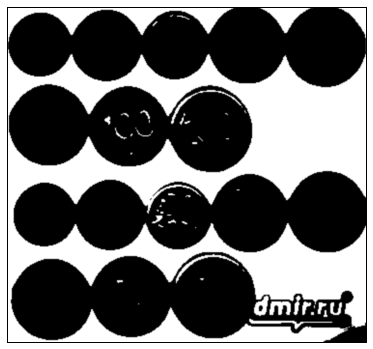
\includegraphics[width=8cm]{Money_3_bin.png} & 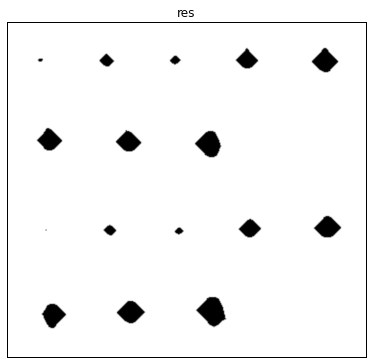
\includegraphics[width=8cm]{Money_3_res.png} \\
		\end{tabular}

		\begin{tabular}{c c}
			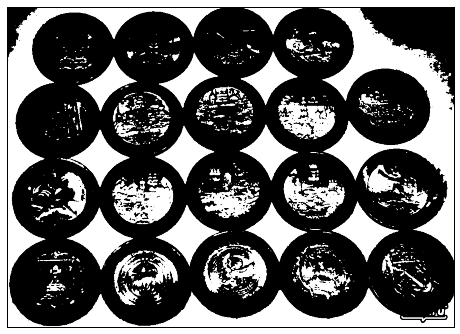
\includegraphics[width=8cm]{Money_4_bin.png} & 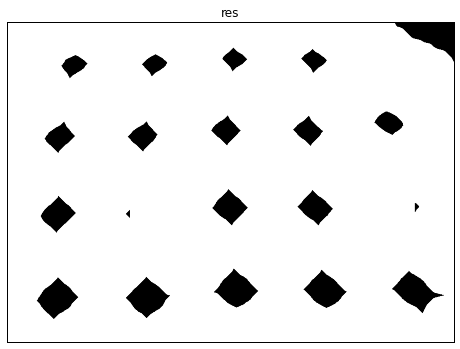
\includegraphics[width=8cm]{Money_4_res.png} \\
			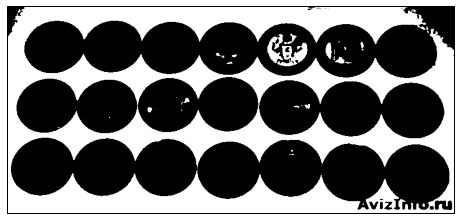
\includegraphics[width=8cm]{Money_6_bin.png} & 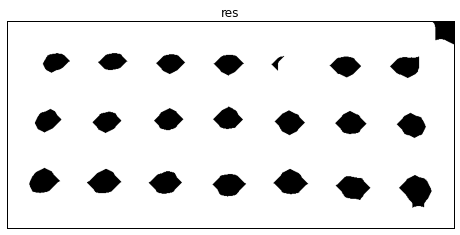
\includegraphics[width=8cm]{Money_6_res.png} \\
			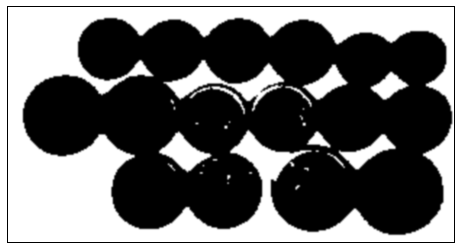
\includegraphics[width=8cm]{Money_7_bin.png} & 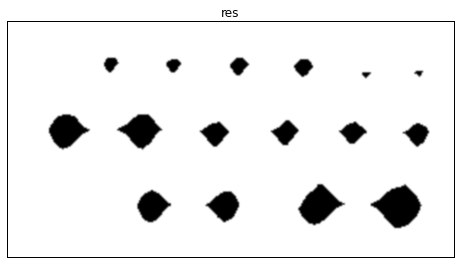
\includegraphics[width=8cm]{Money_7_res.png} \\
			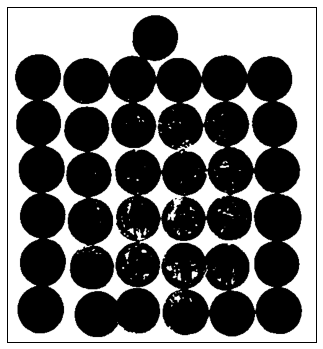
\includegraphics[width=8cm]{Money_8_bin.png} & 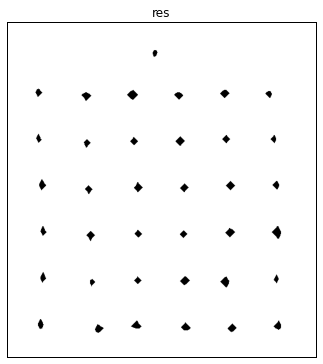
\includegraphics[width=8cm]{Money_8_res.png} \\
		\end{tabular}

		\begin{tabular}{c c}
			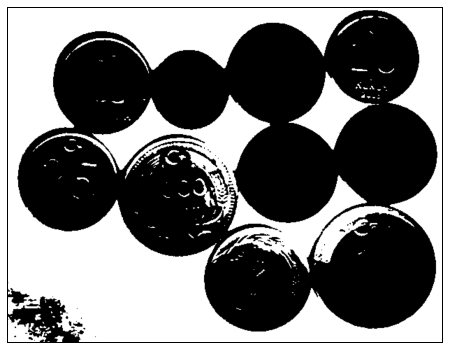
\includegraphics[width=8cm]{Money_9_bin.png} & 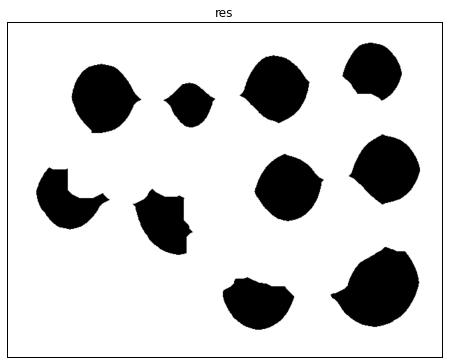
\includegraphics[width=8cm]{Money_9_res.png} \\
			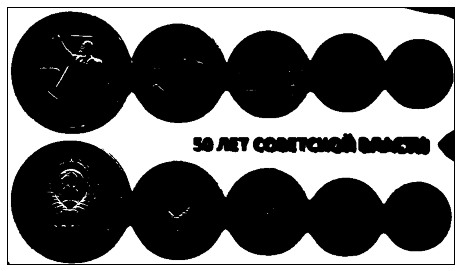
\includegraphics[width=8cm]{Money_10_bin.png} & 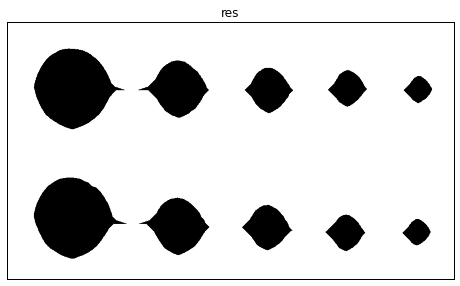
\includegraphics[width=8cm]{Money_10_res.png} \\
			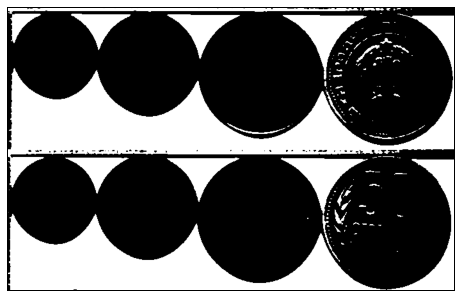
\includegraphics[width=8cm]{Money_11_bin.png} & 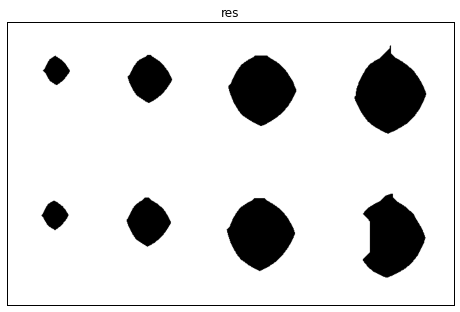
\includegraphics[width=8cm]{Money_11_res.png} \\
			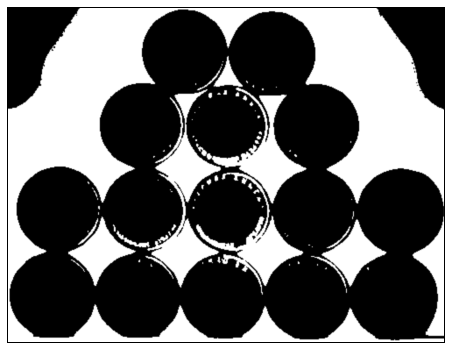
\includegraphics[width=8cm]{Money_12_bin.png} & 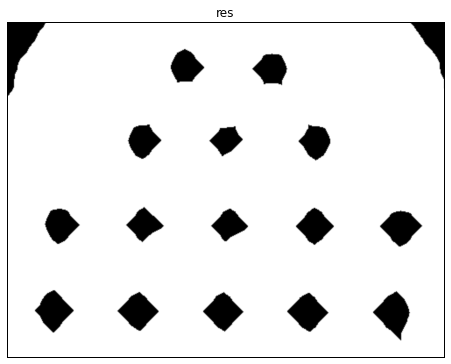
\includegraphics[width=8cm]{Money_12_res.png} \\
		\end{tabular}

		\begin{tabular}{c c}
			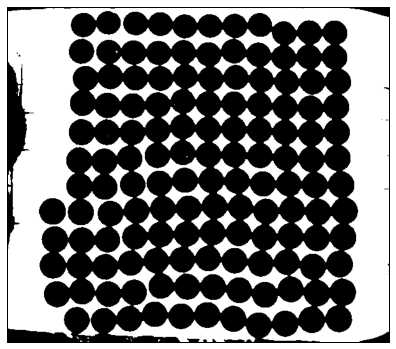
\includegraphics[width=8cm]{Money_15_bin.png} & 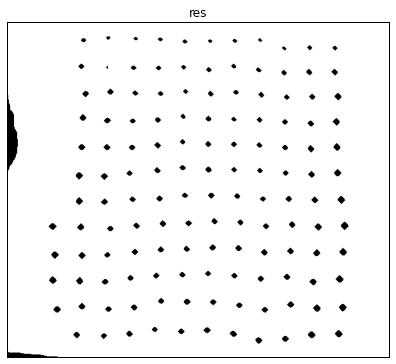
\includegraphics[width=8cm]{Money_15_res.png} \\
			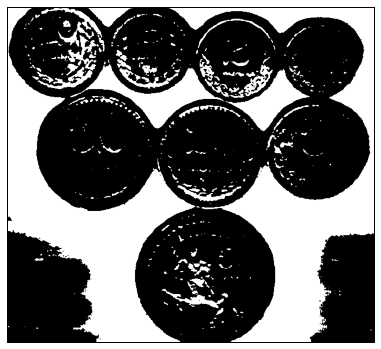
\includegraphics[width=8cm]{Money_16_bin.png} & 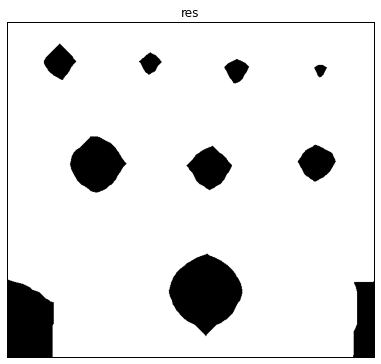
\includegraphics[width=8cm]{Money_16_res.png} \\
		\end{tabular}
		\end{center}

		
\end{document}
